When a visitor first visits the exhibition they have to register using the application, however they most likely do not have the application installed on their phones when first entering the exhibition, so it has to be possible for them to easily get it without having to find it themselves. This can be done using static data storage like \ac{nfc} or \ac{qr}. These two ways of storing information allows us to install/launch the application, identify which exhibition the user is at and other information that might be needed. The following section briefly explains \ac{nfc} and \ac{qr}s and their use. 

\section{NFC}
\ac{nfc} is a way wireless way to transfer data between two \ac{nfc} enabled devices. 
An \ac{nfc} tag is a small data storage unit, which allows you to store small amount of information that can then be transferred to an \ac{nfc} device. 

A standard \ac{nfc} tag can contain around 41 characters, whereas the NTAG203 tags can store around 132 characters\citep{nfccap}. Most of the tags store data in a format called \ac{ndef}, this defines a message format used when transfering information between a device and a tag, or two devices. An \ac{ndef} message consists of one or more of so-called \ac{ndef} records. \autoref{fig:ndef} shows general view of an \ac{ndef} message.

\begin{figure}[H]
\centering
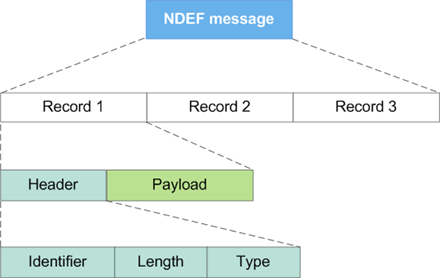
\includegraphics[width=0.8\textwidth]{img/nfcrecord.png}
\caption{View of an NDEF message\citep{ndef}}
\label{fig:ndef}
\end{figure}

An example of a record could be the URL \textit{http://nokia.com}. When reading the \ac{nfc} tag, the following hexa code has to be interpreted: 

\begin{quote}
03 0e d1 01 0a 55 03 6e 6f 6b 69 61 2e 63 6f 6d fe
\end{quote}

Each byte contains some information about what has been scanned \citep{ndef}.

\begin{itemize}
\item 03 - the first byte defines the type of the record. An NDEF record is presented by a 03.
\item 0e - the second byte tells the reader how many bytes the payload consists off.
\item d1 - Each NDEF record is of variable length, but they all have a common format which can be seen on\autoref{fig:binformat}. d1 is binary code representing different information about the record.
\end{itemize}

\begin{figure}[H]
\centering
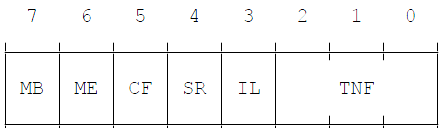
\includegraphics[width=0.8\textwidth]{img/binformat.png}
\caption{NDEF record format\citep{ndef}}
\label{fig:binformat}
\end{figure}

In this example d1 is the binary code \textit{11010001}, each of the numbers represent a flag for true and false, indicating different things about this specific record\citep{ndef}. 

\begin{itemize}
\item MB means "message begin". The flag is set to 1, which means that this is the first record in the \ac{ndef} message.
\item ME means "message end". The flag is set to 1, which means that this is the last record in the \ac{ndef} message. If this is false, then the application knows there are more records coming.
\item CF means "chunked message", An application can be split into multiple chunks and carried in different \ac{ndef} records. If this is the case, each record has the CF flag set to 1 except for the last one which is set to 0.
\item SR means "short record", if the flag is set to 1 it means that the payload length is a single octet. 
\item IL means "identification length", if the flag is 0 then the $ID\_LENGTH$ field is ommited in the record. The $ID\_LENGTH$ indicates the length of the ID field in bytes\citep{ndefformat}.
\item The Type Name Format (TNF) value indicates the structure of the TYPE field. It is a 3-bit value that describes the record type\citep{ndefformat}.
\end{itemize}

When a record like in the example is scanned, the website is launched inside the mobile browser. 

An \ac{ndef} can not only be an URL like in the example, but it could also be a simple textrecord or a package name of an application. 

A text record can contain letters, symbols and numbers. If a record contains is a package name and the tag is scanned, if you have the package installed then the application will launch, else it will take you to the Google Play Store where you can install the application. 

\section{QR code}

A QR code is sort of like a barcode that is seen on groceries at the supermarket, except a normal barcode is only capable of storing 20 digits, where as a \ac{qr} can store up to 7,089 characters. Even if a \ac{qr} is dirty or damaged, it is possible to restore the data due to its error correction capability. However there are limits to how damaged, up to 30\% of the information can be restored. It is also possible to scan a \ac{qr} from any direction  because of the patterns located at the three corners of the code, as seen on \autoref{fig:symbolImage} \citep{qrcode}.

\begin{figure}[H]
\centering
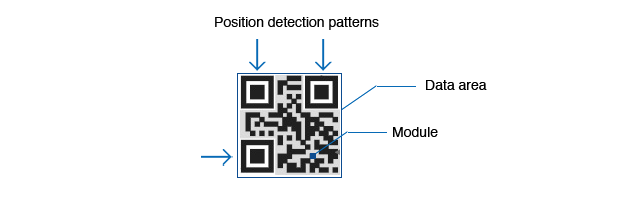
\includegraphics[width=1.5\textwidth]{img/symbolImage.png}
\caption{\ac{qr}\citep{qrcode}}
\label{fig:symbolImage}
\end{figure}

The message data on the code is placed in a zigzag pattern as seen on \autoref{fig:qrplacement} 

\begin{figure}[H]
\centering
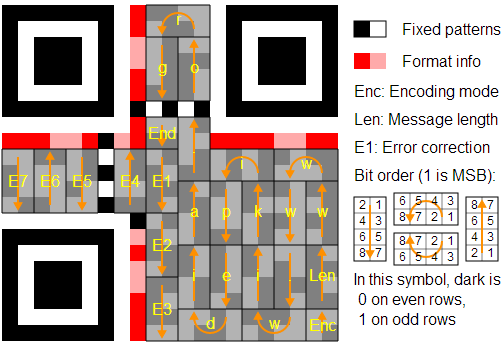
\includegraphics[width=0.8\textwidth]{img/qrplacement.png}
\caption{Zigzag pattern in a \ac{qr}\citep{qrcode1}}
\label{fig:qrplacement}
\end{figure}

The encoding mode consists of four bits, indicating what encoding mode is used and to convey other information. There are a number of indicators, but some of the more common indicators are:

\begin{description}
\item 0001 - Numeric encoding (10 bits per 3 digits)
\item 0010 - Alphanumeic encoding (11 bits per 2 charaters)
\item 0100 - Byte encoding (8 bits per character)
\end{description}

For example, if you were to encode the word "\ac{qr}" in numeric mode, the mode indicator is 0001.

\begin{table}[H]
\centering
\begin{tabular}{|l|l|l|l|}
\hline
\textbf{Encoding} & \textbf{Ver. 1-9} & \textbf{10-26} & \textbf{27-40} \\
\hline
\textbf{Numeric } & 10 & 12 & 14  \\
\hline
\textbf{Alphanumeric} & 9 & 11 & 13 \\
\hline
\textbf{Byte} & 8 & 16 & 16 \\
\hline
\end{tabular}
\caption{Encoding versions}
\label{tab:qrversion}
\end{table}

After the encoding mode, there is a length field that tells how many characters is encoded in the mode specified. The number of bits in the field depends on the encoding and symbol version\citep{qrcode1}. The symbol version, as seen in \autoref{tab:qrversion} can range between 1 an 40. Each version has a different number of modules, modules being the small black and white dots that make up a \ac{qr}\citep{qrversion}. 

\section{Our choice of data storage}
We chose to use \ac{nfc} tags as our way of storing the data. Even though you have to buy the \ac{nfc} tags instead of printing them yourself like you can with QR-codes. The tags are easy to use, you can even have the supplier write them and make them read-only for you. The \ac{nfc} tags are not too expensive, and when buying in bulks some sites even offer a discount up to $25\%$\citep{nfczonen}. 

We also found it to be an inconvenience for the user to have to use the camera to scan a QR code, compared to an NFC-reader which just runs in the background. However the main reason we chose to use \ac{nfc} instead of QR-codes is because a QR code you can scan from far away, and we want to know exactly where a user stands when scanning, so with the short range of \ac{nfc}, we can make sure that the user is actually next to the tag and thereby get their location.